\title{839-1}
\documentclass[12pt,letterpaper]{article}

\usepackage{cvpr}
\usepackage{times}
\usepackage{epsfig}
\usepackage{graphicx}
\usepackage{amsmath}
\usepackage{amssymb}


\newcommand{\mycaption}[3]{{\beforecaption\caption{\label{#1}{\bf #2. } {\em \small #3}}\aftercaption}}

% Include other packages here, before hyperref.

% If you comment hyperref and then uncomment it, you should delete
% egpaper.aux before re-running latex.  (Or just hit 'q' on the first latex
% run, let it finish, and you should be clear).
\usepackage[breaklinks=true,bookmarks=false]{hyperref}

\cvprfinalcopy % *** Uncomment this line for the final submission

\def\cvprPaperID{****} % *** Enter the CVPR Paper ID here
\def\httilde{\mbox{\tt\raisebox{-.5ex}{\symbol{126}}}}

% Pages are numbered in submission mode, and unnumbered in camera-ready
%\ifcvprfinal\pagestyle{empty}\fi
\setcounter{page}{1}
\begin{document}

%%%%%%%%% TITLE
\title{CS 839 Project Stage 1: Information Extraction from Natural Text: \\Extracting Cryptocurrencies from News Articles}

\author{Aishwarya Ganesan\\
{\tt ag@cs.wisc.edu}
% For a paper whose authors are all at the same institution,
% omit the following lines up until the closing ``}''.
% Additional authors and addresses can be added with ``\and'',
% just like the second author.
% To save space, use either the email address or home page, not both
\and
David Liang\\
{\tt david.liang@wisc.edu}
\and 
Viswesh Periyasamy\\
{\tt vperiyasamy@wisc.edu}
}

\maketitle
%\thispagestyle{empty}

\section*{DataSet}
\begin{enumerate}
\item \textbf{Entity type:} The entity type that we decided to extract is \textit{Cryptocurrency}. A few examples of mentions of this entity type include \textit{BitCoin}, \textit{Ethereum}, \textit{Ripple}, \textit{BitCoin Cash}, etc.
\item \textbf{Number of Mentions:} The total number of mentions that we marked up is \textbf{9082}. The total number of negative instances in the data set after pruning is \textbf{243256}.\\
\textbf{Set I:} The number of documents in set I is \textbf{200}, and the number of mentions in set I is \textbf{6080}. \\
\textbf{Set J:} The number of documents in set J is \textbf{100}, and the number of mentions in set J is \textbf{3002}. 
\end{enumerate}
 
\section*{Classifier M}
\begin{figure}[h!]
\centering
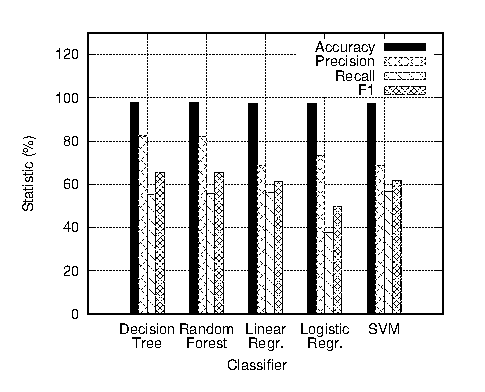
\includegraphics[width=0.5\textwidth]{M_I}
\caption{Initial Cross Validation Performance of different classifiers on set I}
\label{fig1}
\end{figure}

Figure~\ref{fig1} shows the results of performing cross validation with five folds on set I the first time using different classifiers. We tried the following features when we initially ran our classifiers:
\\\indent Word length
\\\indent Number of capital letters in the string
\\\indent Does the string has all capital letters?
\\\indent Does the string contains cash as substring?
\\\indent Does the string contains coin as substring?
\\\indent Is first letter of the word capitalized?
\\\indent Is word surrounded by parentheses?


Based on the results (shown in Figure~\ref{fig1}) we picked \textit{Decision Trees} as the classifier M. The precision, recall, F1 of performing cross validation with M on set I with five folds are \textbf{82.33\%}, \textbf{55.35}\%, and \textbf{65.45}\% respectively.
%the type of the classifier that you selected after performing cross validation on set I *the first time*, and the precision, recall, F1 of this classifier (on set I). This classifier is referred to as classifier M in the description above. 


\section*{Classifier X}
We added more features to improve the performance of the extractor. Some features that we added include:
\\\indent The next string in the sentence that immediately follows the current word.
\\\indent Counts of different characters in the word
\\\indent Check for substrings \textit{ium} and \textit{eum}
\\\indent Check for special characters like forward slash, dash, apostrophe, dot, etc.

Figure~\ref{fig2} shows the results of performing cross validation with five folds on set I using different classifiers after debugging (using set I) and the above features to improve the precision and recall. The type of the classifier that we finally settled on before the rule-based post-processing step is \textit{Random Forest}. 
\begin{figure}[h]
\centering
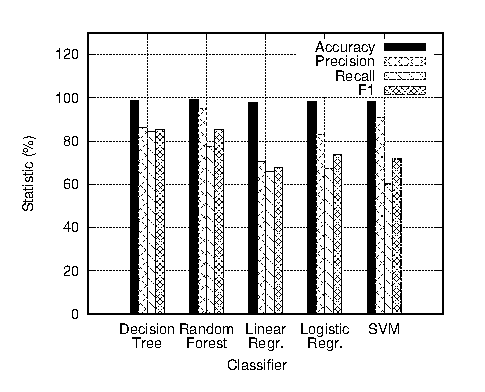
\includegraphics[width=0.5\textwidth]{X_I}
\caption{Cross Validation Performance after debugging different classifiers on set I}
\label{fig2}
\end{figure}

The results of running 5-fold cross validation using Random Forest on the test set J are as follows:\\
Accuracy: 99.31\%\\
Precision: 96.86\%\\
Recall: 82.21\%\\
F1: 88.93\%\\


\section*{Final Classifier Y}
\textbf{Rule-Based Post-Processing:} We added a set of most common crypto currencies like \textit{BitCoin}, \textit{Ethereum}, etc., into a whitelist. If a word we are trying to classify is part of the whitelist, we mark it a cryptocurrency. 

The final classifier Y  is \textit{Random Forest} along with the above post processing. The final results of running Y on the test set J are as follows:\\
Random Forest accuracy: 99.33\%\\
Precision: 96.86\%\\
Recall: 82.21\%\\
F1: 88.93\%\\
%Report the precision, recall, F1 of classifier Y (see description above) on set J. This is the final classifier (plus rule-based post-processing if you have done any). 


{\small
%\bibliographystyle{plain}
%\bibliography{egbib}
}

\end{document}
